%Créé par Samuel Tremblay en collaboration avec Jean-Raphaël Carrier et Claudine Allen
%Dernière modification JRC: 13 janvier 2014
%Élimination du labo de résistivité des matériaux (IV) à la fin de l'ère JRC => renumérotation XII -> XI puis passé à optionnel pour finalement disparaître en pandémie COVID-19
%Dernière modification CA: 2 novembre 2020
%
\documentclass[12pt,oneside,letterpaper]{article}

\usepackage[utf8]{inputenc}
\usepackage[T1]{fontenc}
\usepackage[canadien]{babel}
\usepackage{lmodern}
\usepackage{graphicx}
\usepackage[letterpaper]{geometry}
\usepackage[americanvoltages,americancurrents]{circuitikz}
\usetikzlibrary{babel}
\usepackage{setspace}
\usepackage{color}
\usepackage{caption}
\usepackage{subfig}
\usepackage{hyperref}
\usepackage[all]{hypcap}

\usepackage{sistyle}
\usepackage{csquotes}

\usepackage{hyperref}
\usepackage[all]{hypcap}



\addto\captionsfrench{\def\tablename{Tableau}}
\linespread{1.3}
\setcounter{secnumdepth}{0}
\captionsetup{font=small,labelfont=bf,margin=0.1\textwidth}
\pagestyle{myheadings}
\markboth{GPH-2006/PHY-2002~---~Projet~de~conception}{GPH-2006/PHY-2002~---~Projet~de~conception}



\begin{document}



\title{\singlespace{\textbf{Complément}\\Initiation à la simulation de circuits}}
\author{Claudine Allen \& Alicia Talbot-Lanciault}
\date{}
\maketitle



\section{}

Dans le cadre de projets de plus grande envergure, il est souvent pertinent de
faire des tests préliminaires des circuits électroniques en observant leur comportement
à l’aide d’un simulateur de circuits. Le logiciel professionnel recommandé par
le Département de génie électrique et de génie informatique de l’Université Laval
est Altium http://www.altium.com/, mais nous vous proposons ici une alternative
gratuite de simulateur en ligne programmé par Paul Falstad et adapté en langage
JavaScript par Iain Sharp. Celui-ci est disponible directement via votre navigateur
à l’adresse http://falstad.com/circuit/. Ce simulateur est moins performant et
loin d’être aussi complet qu’Altium, mais il est cependant plus simple et intuitif à
utiliser avec de bonnes visualisations pédagogiques. La figure 1 présente l’exemple
de circuit proposé à l’arrivée sur le site Internet de Paul Falstad.

\begin{figure}
    \centering
    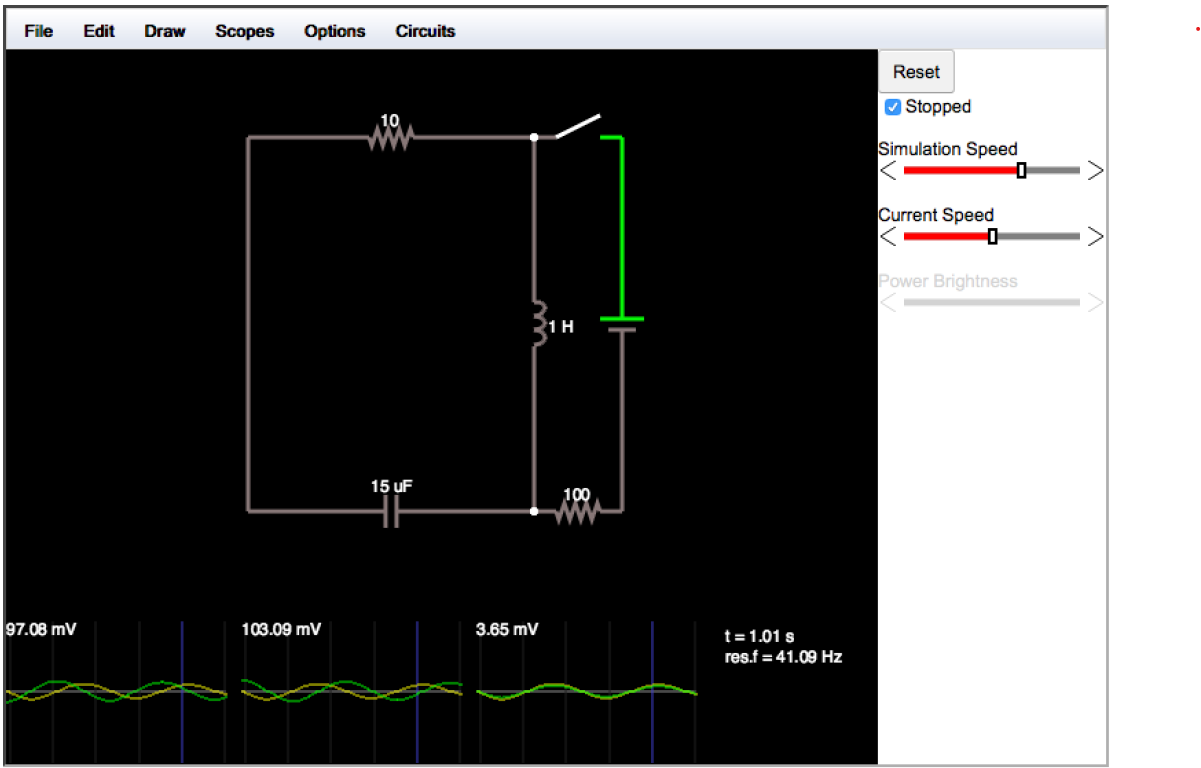
\includegraphics[width=0.5\linewidth]{Labos-Complements/Falstad-simulation circuit RLC.png}
    \caption{Simulation d’un circuit RLC avec oscilloscopes dans le bas
de l’image montrant le signal en fonction du temps. Capture d’écran de
la page Web de Paul Falstad.\footnote{\label{airtable}{P. Falstad, "Electronic Circuit Simulator" <\url{<http://falstad.com/circuit/}>.}}}
    \label{Figure 1}
\end{figure}

\section{Fonctionnalités intéressantes}
\subsection{Dessiner un circuit}

Le logiciel offre une vaste sélection de composants électroniques. Dans l’onglet
Draw, il est possible de sélectionner une résistance, une source de tension ou de courant,
alternative ou non, un condensateur, une inductance, un transistor... Lorsqu’un
composant est sélectionné, il est possible de régler ses caractéristiques en doublecliquant
dessus. Il est important de relier les composants par leurs bouts ou par
des fils. Chaque branchement doit être fait sur un noeud. Il n’est donc pas possible
d’aller brancher un composant au centre d’un long fil. Si vous faites des mauvais
branchements, un signalement apparaîtra au bas de la fenêtre.



\subsection{Observer un circuit}

Grâce au simulateur, vous pourrez observer le comportement de votre circuit et
son évolution dans le temps. L’onglet Options vous permet, entre autres, d’afficher
le courant, la tension et la puissance dans le circuit. Vous pouvez également fixer la
vitesse de la simulation, du courant, réinitialiser votre circuit ou faire une pause à la
simulation à l’aide des fonctionnalités à la droite de la fenêtre. Si vous souhaitez suivre
le comportement d’un composant en particulier, vous pouvez glisser votre curseur sur
le composant et observer le courant qui le traverse et la différence de potentiel à ses
bornes. Il est également possible d’avoir un suivi plus complet du signal traversant un
composant à l’aide de la fonctionnalité view scope obtenue en effectuant un clic droit
sur le composant choisi. Cette dernière fonctionnalité peut s’avérer très intéressante
dans la comparaison des signaux traversant différents composants du circuit.


\subsection{Enregistrer un circuit}

Si vous souhaitez réutiliser un circuit, il est possible de le conserver en exportant
le code comme un url ou comme un fichier .tex. Ces fonctionnalités sont disponibles
dans l’onglet File.



\end{document}

